\documentclass[11pt,letterpaper]{article}
\usepackage[utf8]{inputenc}
\usepackage[T1]{fontenc}
\usepackage{mathptmx}
\usepackage[letterpaper,left=1.25in,right=1.25in,top=1.2in,bottom=1.2in,headheight=14pt]{geometry}
\usepackage{microtype}
\usepackage{amsmath,amssymb,amsthm,mathtools,bm}
\usepackage{graphicx,booktabs,array,multirow,float}
\usepackage{xcolor}
\usepackage{enumitem}
\usepackage[labelfont=bf,labelsep=colon,font=small,skip=4pt]{caption}
\usepackage{subcaption}
\usepackage{fancyhdr}
\usepackage{titlesec}
\usepackage{listings}
\usepackage{tikz}
\usetikzlibrary{arrows.meta,positioning,calc}
\usepackage[authoryear,round]{natbib}
\definecolor{linkcol}{HTML}{2B3A8F}
\usepackage[colorlinks=true,linkcolor=linkcol,citecolor=linkcol,urlcolor=linkcol]{hyperref}
\usepackage[capitalise,noabbrev]{cleveref}

\pagestyle{fancy}\fancyhf{}
\lhead{\small Technical report.}
\cfoot{\small\thepage}
\renewcommand{\headrulewidth}{0.5pt}
\setlength{\parskip}{4pt plus 1pt}\setlength{\parindent}{0pt}
\titleformat{\section}{\large\bfseries}{\thesection}{0.8em}{}
\titleformat{\subsection}{\normalsize\bfseries}{\thesubsection}{0.8em}{}
\titleformat{\subsubsection}{\normalsize\bfseries\itshape}{\thesubsubsection}{0.8em}{}
\titlespacing*{\section}{0pt}{16pt}{6pt}\titlespacing*{\subsection}{0pt}{12pt}{4pt}
\setlist{itemsep=1pt,topsep=3pt}
\setlength{\emergencystretch}{2em}

\theoremstyle{definition}
\newtheorem{definition}{Definition}
\theoremstyle{remark}
\newtheorem{remark}{Remark}

\lstset{basicstyle=\ttfamily\small,breaklines=true,frame=single,framerule=0.3pt,
  xleftmargin=4pt,xrightmargin=4pt,columns=fullflexible,keepspaces=true,showstringspaces=false}

% title block: \reporttitle{title}{subtitle}{authors}{affiliation line}
\newcommand{\reporttitle}[4]{%
\begin{center}
{\LARGE\bfseries #1\\[4pt]
\Large #2\par}
\vspace{1.4em}
{\bfseries\color{linkcol}\large #3}\\[0.4em]
{\small #4}\par
\vspace{1.2em}
\end{center}}
\newcommand{\abstractblock}[1]{%
\begin{center}\textbf{Abstract}\end{center}
\vspace{-0.4em}
\begin{quote}\small #1\end{quote}
\vspace{0.4em}}

\usepackage{pgfplots}\pgfplotsset{compat=1.17}
\begin{document}
\reporttitle{A Multi-Stage Thermoelectric Refrigerator}{PID Control, Printed Thermal Hardware and Power-Electronics Wiring\\ for a Compressor-Less Cooler}{Juan Fernando Castaño \quad with the Falcons team}{N.\,Serikbayev, A.\,Akhmetov, Y.\,Bekbash, N.\,Aitmukhanbetov, R.\,Villarreal, R.\,Valdivia\\ New York University Abu Dhabi \quad $\cdot$ \quad ENGR-UH 3110 Instrumentation, Sensors and Actuators \quad $\cdot$ \quad \href{mailto:jfc9577@nyu.edu}{jfc9577@nyu.edu}}

\abstractblock{Seven students designed, built and controlled a compressor-less cooler driven by Peltier (TEC1-12706) modules, an Arduino PID loop and PWM power electronics. The first build failed in two ways: the hot sides of the modules saturated thermally, and the switching MOSFETs overheated. We redesigned the thermal stack (a printed fan and TEC platform in three generations, with PLA kept out of the heat paths, cork frames, polyurethane-foam sealing and a condensate collector), the power stage (an analysis of the IRF520 gate drive, two MOSFETs per module and a separate acrylic MOSFET box) and the wiring. Step-response trials of three PID gain orderings settled on $K_p=100$, $K_i=0.1$, $K_d=1000$. The cooler pulled a 24.0\,\textdegree C chamber down to a stable 18.0\,\textdegree C in the fan-mixed zone in about 72 minutes, with a local minimum of about 4\,\textdegree C near the cold plate. It did not reach the sub-10\,\textdegree C goal. A code review found that the original sketch swapped the setpoint and input arguments of the PID call, a working reverse-acting trick with a side effect on the derivative term; a conventional reference sketch is included. No controlled comparison of print materials was run.}

\section{Introduction}
A thermoelectric cooler has no moving refrigerant and no compressor, which makes it attractive for a small portable chamber and unattractive for efficiency. The course project was to build one around Peltier modules, an Arduino and a PID loop, and to bring a chamber well below ambient. We set a goal of below 10\,\textdegree C.

Two questions organised the work.

\textbf{Question 1: what limits how cold the chamber gets?} A Peltier module pumps heat from its cold face to its hot face, and its pumping capacity falls as the hot face warms. Everything that follows, the platform, the fans, the materials and the electronics, is about keeping the hot side cool and the modules fully driven.

\textbf{Question 2: can a simple PID loop control a plant with a long time constant and a hard nonlinearity?} The chamber takes tens of minutes to move a degree, and the actuator is saturating.

\textbf{What we find.} The chamber reached a stable 18.0\,\textdegree C from 24.0\,\textdegree C, short of the goal. In order of impact, the shortfall comes from the heat-rejection capacity of the hot-side stack, from a MOSFET drive that limited the usable current, and, initially, from poor air mixing inside the chamber. The first two were diagnosed during the project; the second has an identified fix that we did not build.

\textbf{Contributions.} We do not propose a new design. We contribute:
\begin{enumerate}
\item A step-response study of three PID gain orderings and the gains we settled on (\cref{sec:pid}).
\item A three-generation printed platform and the material decisions behind it (\cref{sec:print}).
\item A diagnosis of the MOSFET failure from the gate-drive limits of the IRF520, and the power stage that came out of it (\cref{sec:wiring}).
\item A review of the control code that found a swapped argument order in the PID call (\cref{sec:review}).
\item Test results with their limits (\cref{sec:results}).
\end{enumerate}

\textbf{Organisation.} \Cref{sec:background} gives background, \cref{sec:system} the system, and \cref{sec:pid,sec:print,sec:wiring} the three development areas. \Cref{sec:results} presents the results and \cref{sec:discussion} states what they establish.

\section{Background}\label{sec:background}
\textbf{Peltier cooling.} A thermoelectric module moves heat in proportion to current, while Joule heating inside it grows with the square of current and conduction carries heat back from hot to cold. The net pumping capacity therefore peaks at a moderate current and falls as the temperature difference between the faces grows \citep{goldsmid2010,rowe2006}. Published mini-refrigerators of this kind are usually studied through their coefficient of performance and their hot-side cooling \citep{elnaggar2024,beck2018}.

\textbf{PID control.} A PID loop acts on the error between setpoint and measurement through proportional, integral and derivative terms \citep{astrom1995}. Practical implementations add output limits, protection against integrator wind-up and, in the common Arduino library, derivative action on the measurement to avoid kicks when the setpoint changes \citep{beauregard2011,dewesoft2024}.

\textbf{Switching a TEC.} A TEC is a resistive load of several amperes. An N-channel MOSFET switched by PWM is the usual driver, and it conducts efficiently only when its gate is driven hard enough. The IRF520 reaches its quoted on-resistance of 0.27\,$\Omega$ at a gate voltage of about 10\,V \citep{irf520}, a point raised on hobbyist forums as a reason not to drive it from 5\,V logic \citep{forum2021}.

\section{System Overview}\label{sec:system}
The cooler is a commercial passive cooler body modified with a thermally isolated hot-side platform (\cref{fig:cad}). Heat is pumped from the cold plate through the TEC modules into heatsinks blown clear by fans. An Arduino reads the chamber temperature, runs the PID loop and sets the TEC drive through PWM-switched MOSFETs (\cref{fig:arch}).
\begin{figure}[t]\centering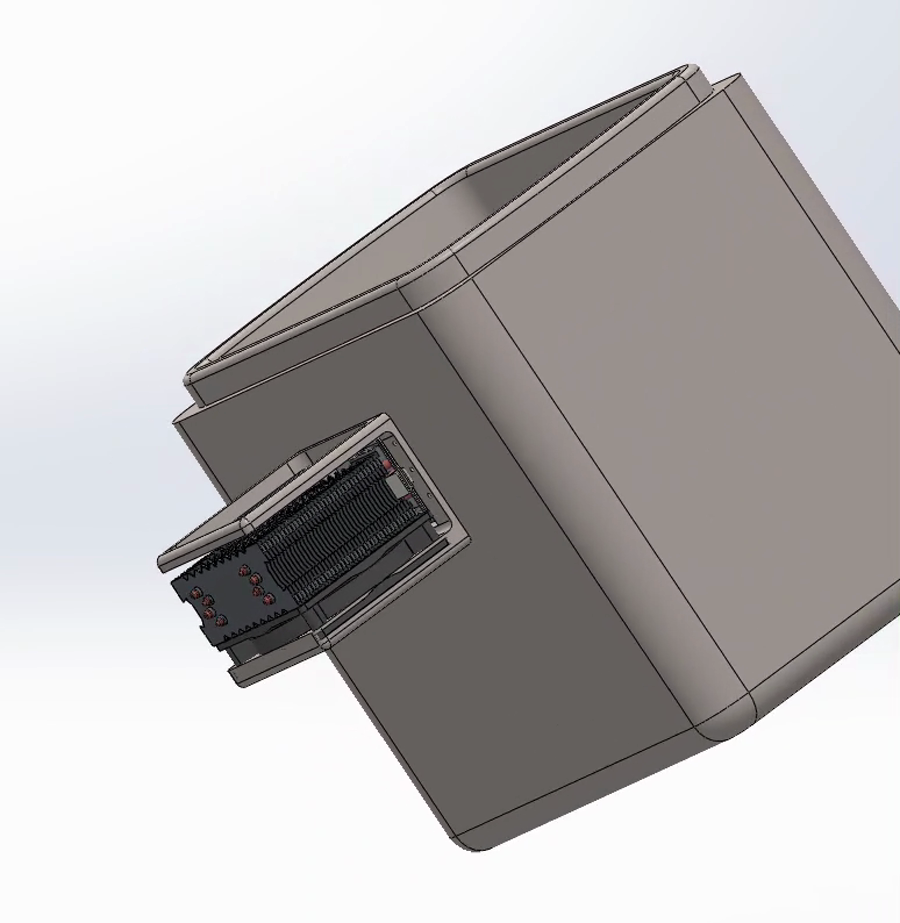
\includegraphics[width=0.55\linewidth]{figures/cad_model.png}
\caption{CAD model of the cooler body with the TEC and heatsink stack mounted in the side wall. An animation of the model is included in the repository.}\label{fig:cad}
\end{figure}
\begin{figure}[t]\centering
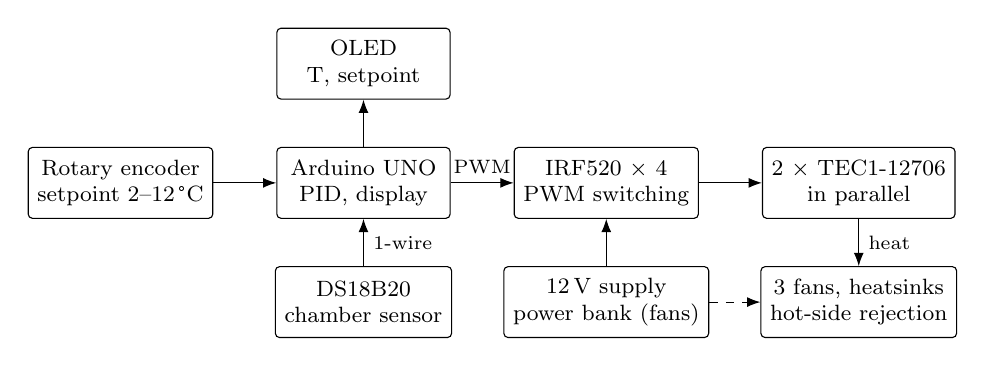
\begin{tikzpicture}[node distance=6mm and 8mm,box/.style={draw,rounded corners=1.5pt,minimum height=9mm,minimum width=22mm,align=center,font=\footnotesize},>=Latex]
 \node[box] (enc) {Rotary encoder\\setpoint 2--12\,\textdegree C};
 \node[box,right=of enc] (ard) {Arduino UNO\\PID, display};
 \node[box,right=of ard] (mos) {IRF520 $\times$ 4\\PWM switching};
 \node[box,right=of mos] (tec) {2 $\times$ TEC1-12706\\in parallel};
 \node[box,below=of ard] (ds) {DS18B20\\chamber sensor};
 \node[box,below=of mos] (psu) {12\,V supply\\power bank (fans)};
 \node[box,below=of tec] (fan) {3 fans, heatsinks\\hot-side rejection};
 \node[box,above=of ard] (oled) {OLED\\T, setpoint};
 \draw[->] (enc)--(ard); \draw[->] (ard)--(mos) node[midway,above,font=\scriptsize]{PWM}; \draw[->] (mos)--(tec);
 \draw[->] (ds)--(ard) node[midway,right,font=\scriptsize]{1-wire}; \draw[->] (ard)--(oled);
 \draw[->] (psu)--(mos); \draw[->] (tec)--(fan) node[midway,right,font=\scriptsize]{heat};
 \draw[->,dashed] (psu) -- (fan);
\end{tikzpicture}
\caption{Functional architecture of the final prototype.}\label{fig:arch}
\end{figure}

\section{PID Temperature Control}\label{sec:pid}
\subsection{Loop and implementation}
The chamber temperature $T$ is compared with the setpoint $T_{sp}$; the controller output $u\in[0,255]$ is written with \texttt{analogWrite} to the MOSFET gate lines. We used the \texttt{PID\_v1} library in automatic mode with output limits 0--255, an adjustable setpoint (initially 5\,\textdegree C) and a 100\,ms display and serial refresh. The plant has a large thermal time constant and a hard nonlinearity: pumping capacity falls as the hot side warms.
\begin{table}[t]\centering\small
\begin{tabular}{@{}llll@{}}\toprule
Parameter & Value & Parameter & Value\\\midrule
$K_p$ & 100 & Output range & 0--255 (8-bit PWM)\\
$K_i$ & 0.1 & Sensor & DS18B20, 1-wire, pin 2\\
$K_d$ & 1000 & PWM pin & 3\\\bottomrule
\end{tabular}
\caption{Final gains and wiring of the control loop.}\label{tab:gains}
\end{table}

\subsection{Tuning study}
Instead of treating the gains as plug-and-play, we ran step-response trials in three deliberately unbalanced regimes and logged the PWM output. The shape of each failure told us which term to reduce (\cref{fig:pid,tab:orderings}).
\begin{figure}[t]\centering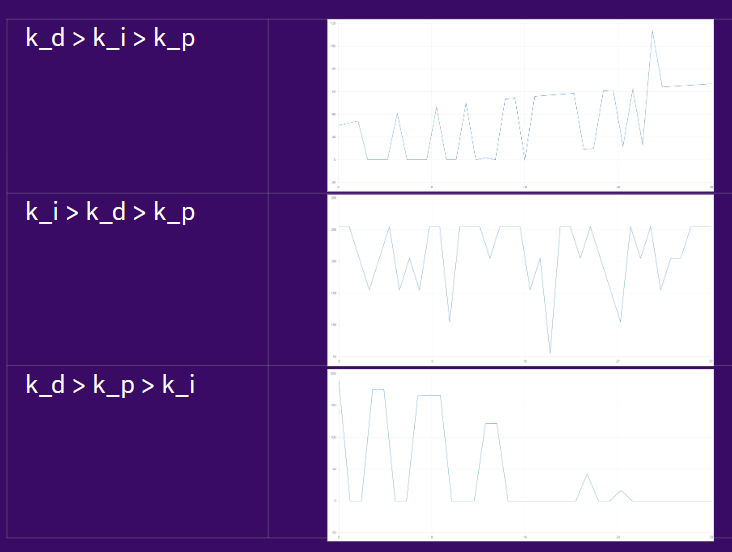
\includegraphics[width=0.62\linewidth]{figures/pid_kcases.png}
\caption{PWM output traces for the three gain orderings tested.}\label{fig:pid}
\end{figure}
\begin{table}[t]\centering\small
\begin{tabular}{@{}lp{2.2in}p{2in}@{}}\toprule
Ordering & Observed behaviour & Diagnosis\\\midrule
$K_d>K_i>K_p$ & Erratic PWM, large jumps & Weak proportional action; derivative dominates\\
$K_i>K_d>K_p$ & Large slow oscillations, repeated overshoot & Integral wind-up; loop blind to the instantaneous error\\
$K_d>K_p>K_i$ & Over-damped, setpoint never reached & Output choked off; integral too small to remove the offset\\\bottomrule
\end{tabular}
\caption{Gain-ordering experiments.}\label{tab:orderings}
\end{table}
We settled on a high proportional gain for fast response to large errors, a very small integral gain to avoid wind-up on a plant that takes tens of minutes to move, and a derivative gain to damp overshoot near the setpoint.

\subsection{A review of the implementation}\label{sec:review}
Reviewing the code while writing this report we noticed that the sketch passes the setpoint as the library's \emph{input} and the measured temperature as its \emph{setpoint}: \texttt{PID myPID(\&setpoint, \&output, \&input, \ldots, DIRECT)}. This is a legitimate way to get a reverse-acting loop, with error $T-T_{sp}$ and more cooling when warm, and it worked. Its side effect is that the library's derivative-on-measurement term then acts on the setpoint and not on the temperature, so the derivative gain mainly produced a kick when the user turned the encoder. The explanation we gave at the time for the erratic regime, derivative action amplifying sensor noise, should therefore be re-tested with the conventional form, \texttt{PID(\&input, \&output, \&setpoint, \ldots, REVERSE)}. The reference sketch in the repository uses that form.

Other changes would improve the loop: a non-blocking DS18B20 read with a short moving-average filter (the sensor resolves 0.0625\,\textdegree C, and one count of derivative at $K_d=1000$ is large), integral clamping tied to the output limits, and gain search from logged step responses in place of manual trials.

\section{Printed Thermal Hardware and Materials}\label{sec:print}
Heat rejection was the central problem, so most of the mechanical effort went into the hot-side platform that holds the TEC stack, the fans and the electronics, and into stopping heat from leaking back.

\subsection{Platform, three generations}
\begin{figure}[t]\centering
\begin{subfigure}{0.50\linewidth}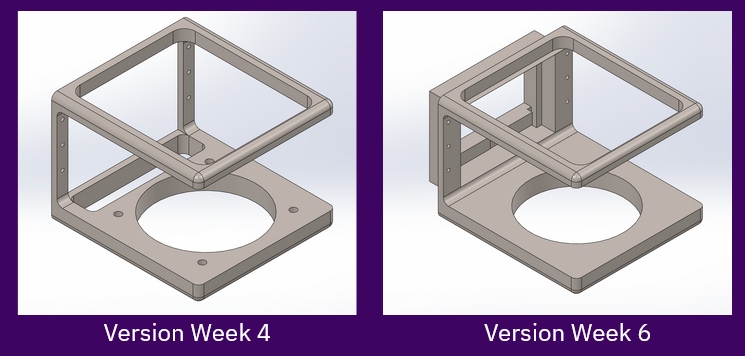
\includegraphics[width=\linewidth]{figures/platform_w4_w6.png}\caption{Week 4 and Week 6 versions (CAD).}\end{subfigure}\hfill
\begin{subfigure}{0.22\linewidth}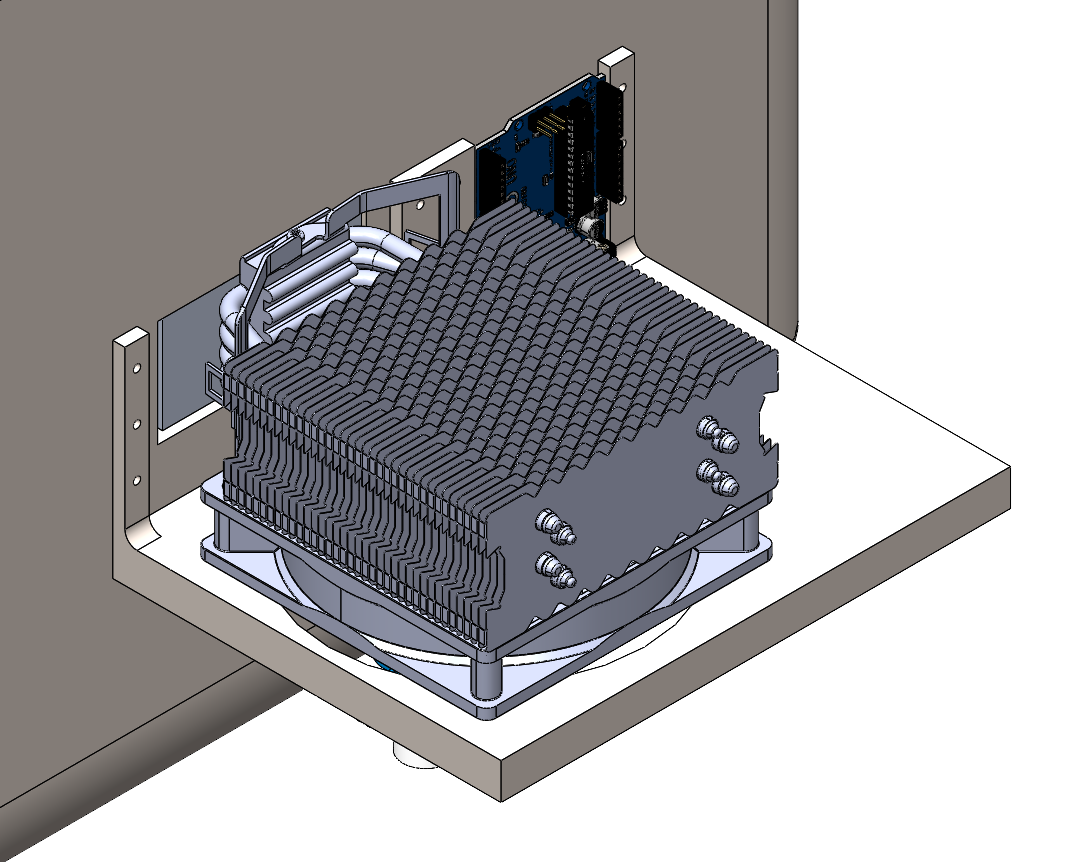
\includegraphics[width=\linewidth]{figures/cad_platform.png}\caption{Final platform.}\end{subfigure}\hfill
\begin{subfigure}{0.22\linewidth}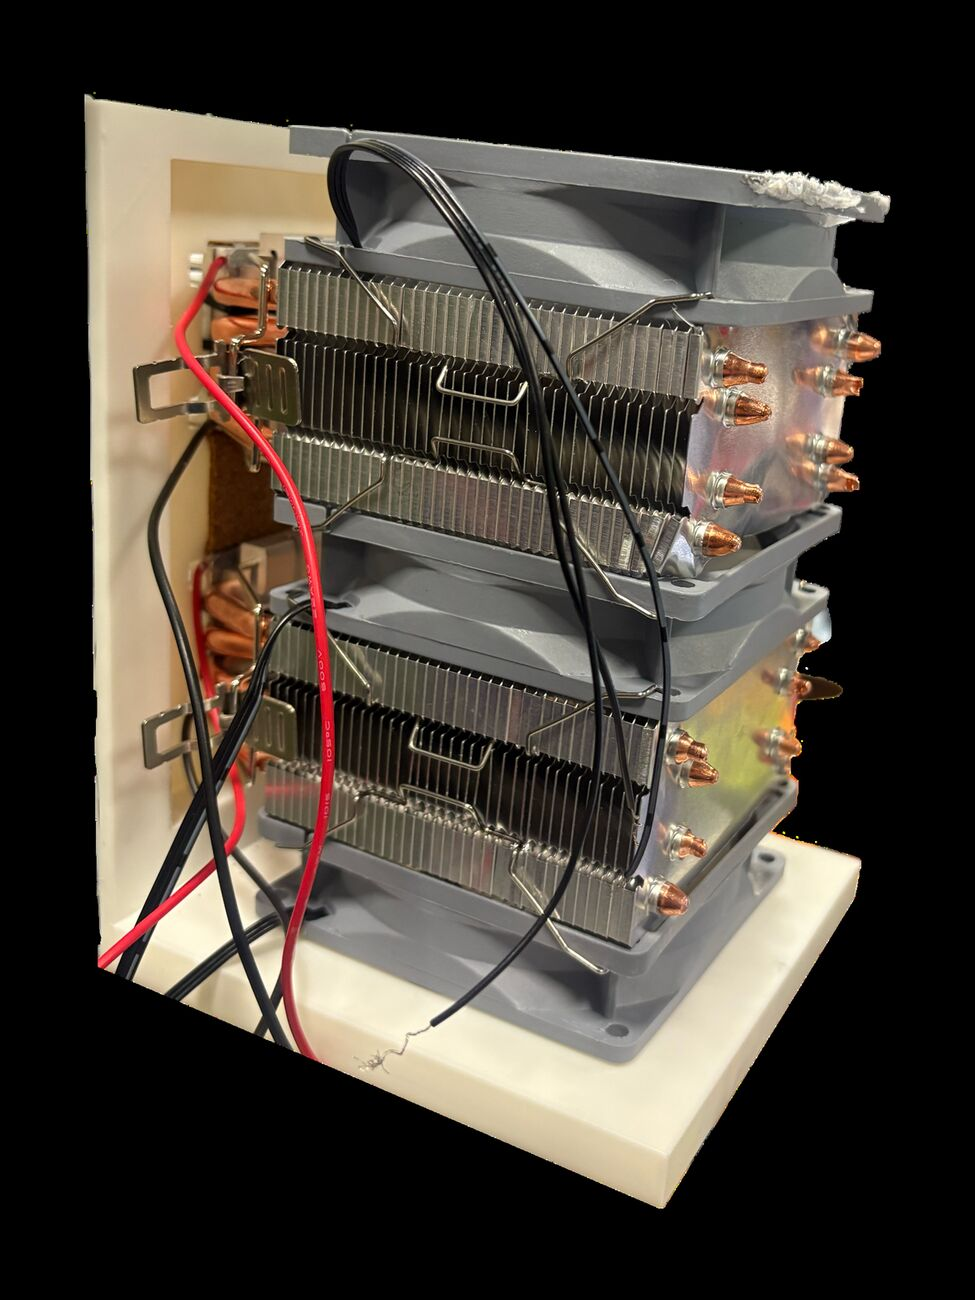
\includegraphics[width=\linewidth]{figures/platform_final.jpg}\caption{Printed and assembled.}\end{subfigure}
\caption{Evolution of the TEC platform.}\label{fig:platform}
\end{figure}
The first version housed the fan and electronics in a closed box. It looked tidy but trapped the TEC heat, warming the cooler and the MOSFETs, and we rejected it after analysis. The second version, from week 6, used an open platform with one fan, a shared metal plate and two series pairs of stacked TECs, with cable channels. In the final version the shared plate was removed: there is one square plate per TEC, two TECs in parallel, one fan per module in direct contact with the plate, all fans blowing the same way, a larger upper compartment and denser infill on the structural side. Direct contact removed interfaces that had added thermal resistance.

\subsection{Material decisions}
Printed PLA softens near 60\,\textdegree C, so no heat-bearing path touches it directly, and platform walls use a higher infill than non-structural parts. Cork frames around the TECs insulate and tolerate temperature, letting the stack run hot without deforming the PLA and tightening the fit. Three packs of thermal paste went between plate, TECs, fins and fans; because the mounting is horizontal and gravity loosened the joints, cable ties clamp the stack. Gaps around the platform, drilled holes and TEC fins were sealed with polyurethane foam, accepting a small loss of fin area for fewer leaks. Enclosures and shelves are 3\,mm laser-cut acrylic with finger joints, cut from DXF layouts, with cardboard test cuts first to avoid wasting acrylic.

\subsection{Structural check of the platform support}
A static study of the platform support bracket under the distributed load of the TEC stack (\cref{fig:fea}) showed small displacements. An animation of the study is included in the repository.
\begin{figure}[t]\centering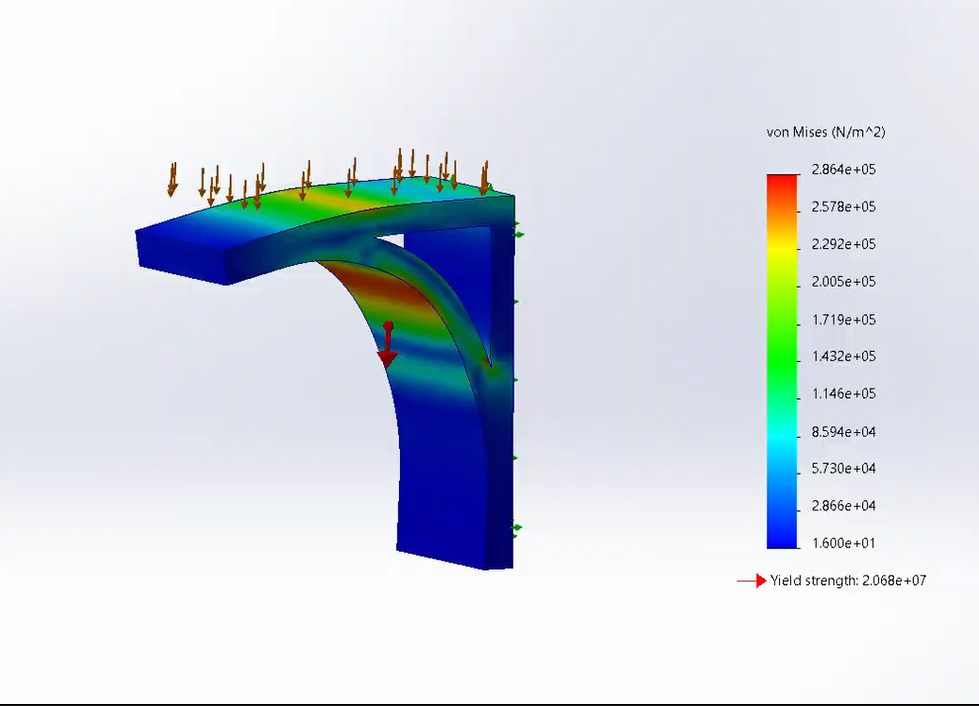
\includegraphics[width=0.55\linewidth]{figures/fea.png}
\caption{Static analysis of the platform support bracket under the distributed load of the TEC stack.}\label{fig:fea}
\end{figure}

\subsection{Condensate collection}
The cold side condenses water, so a printed funnel and tank with a drain valve collect it. The first container did not match the valve that was delivered, so it was redesigned with a slanted floor that drains completely, tested with poured water, then painted and glued in place with the opening sealed with foam (\cref{fig:water}). The control and MOSFET enclosures are laser-cut acrylic, and the supply is mounted on reused filament spools (\cref{fig:encl}).
\begin{figure}[t]\centering
\begin{subfigure}{0.30\linewidth}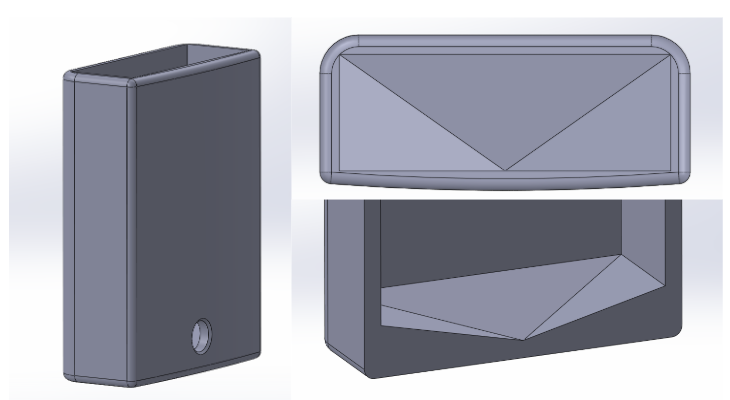
\includegraphics[width=\linewidth]{figures/water_v1.png}\caption{First CAD.}\end{subfigure}\hfill
\begin{subfigure}{0.30\linewidth}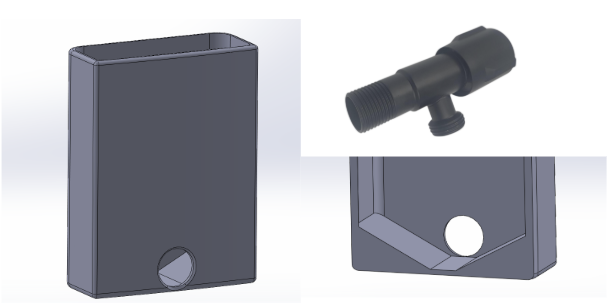
\includegraphics[width=\linewidth]{figures/water_final.png}\caption{Final, with valve.}\end{subfigure}\hfill
\begin{subfigure}{0.17\linewidth}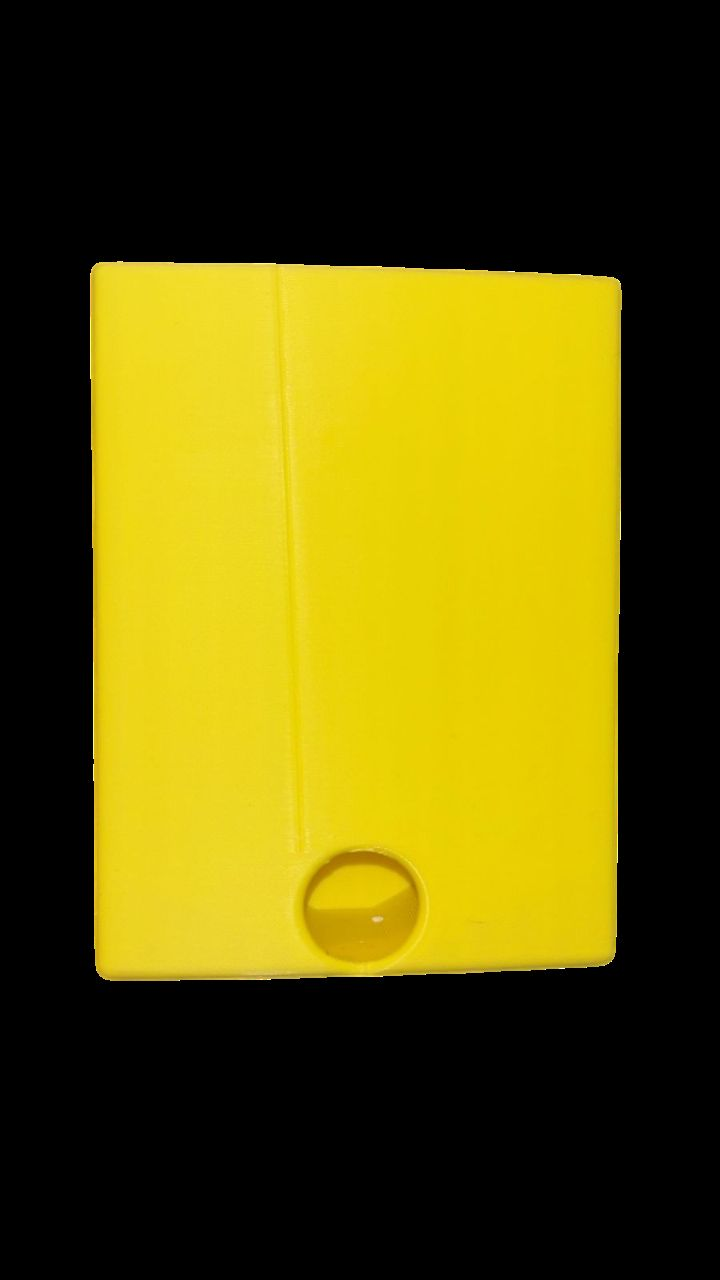
\includegraphics[width=\linewidth]{figures/water_var_a.png}\caption{Print.}\end{subfigure}\hfill
\begin{subfigure}{0.17\linewidth}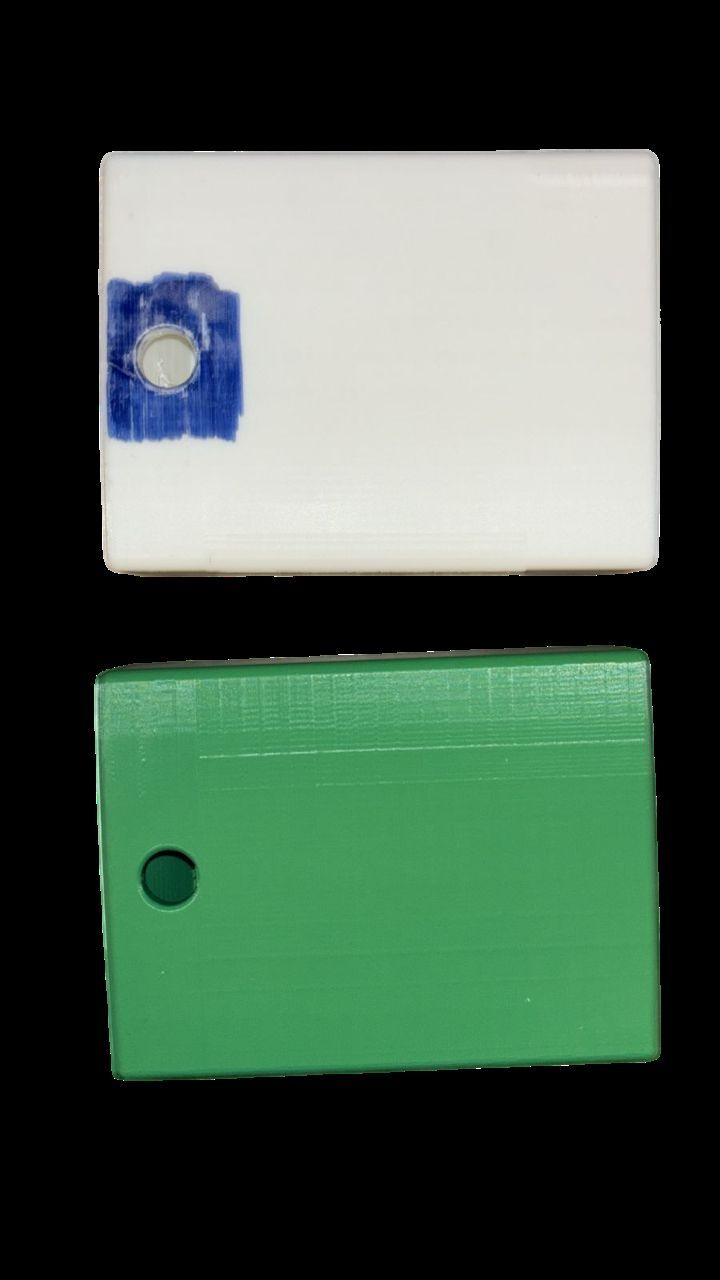
\includegraphics[width=\linewidth]{figures/water_var_b.jpg}\caption{Final.}\end{subfigure}
\caption{Condensate container iterations.}\label{fig:water}
\end{figure}
\begin{figure}[t]\centering
\begin{subfigure}{0.32\linewidth}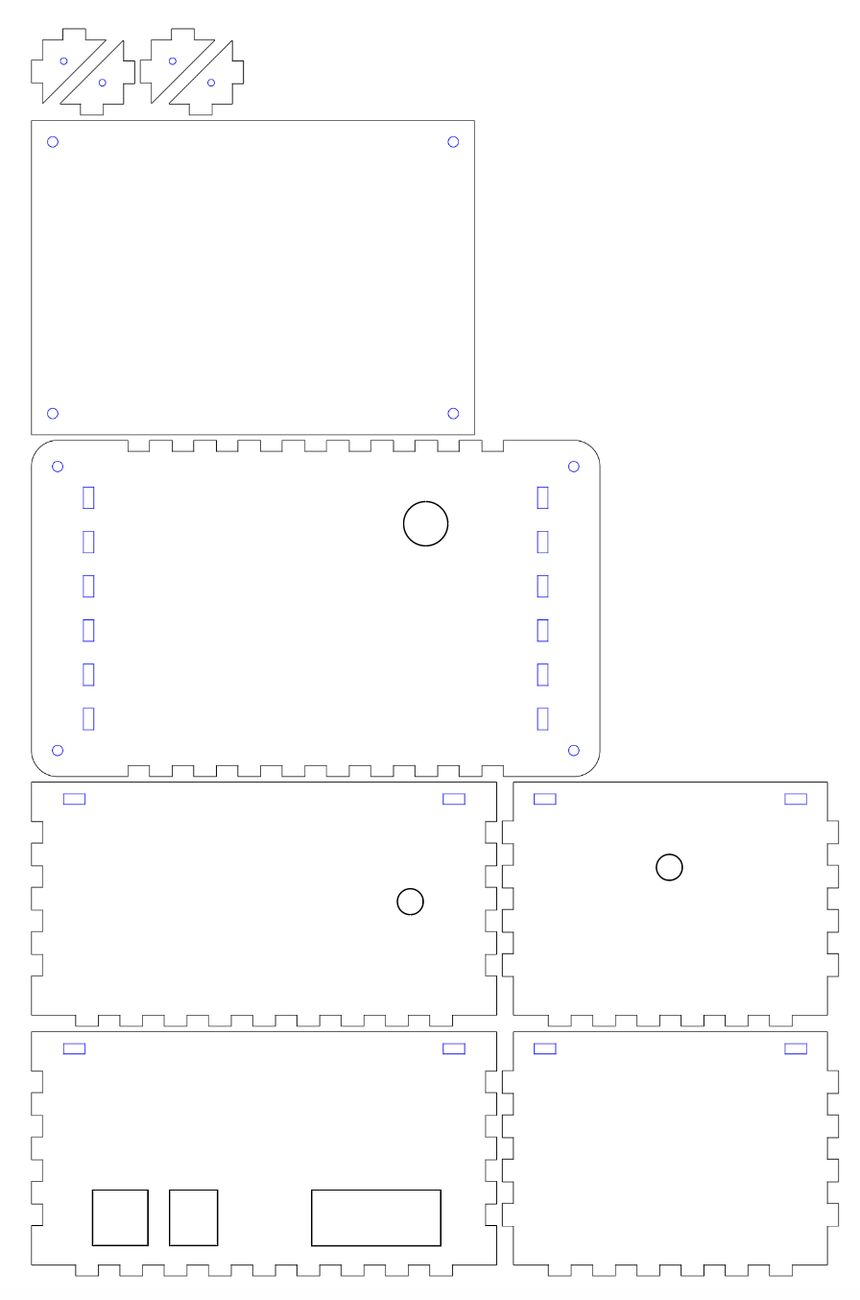
\includegraphics[width=\linewidth]{figures/dxf_circuit_box.jpg}\caption{Control box layout.}\end{subfigure}\hfill
\begin{subfigure}{0.32\linewidth}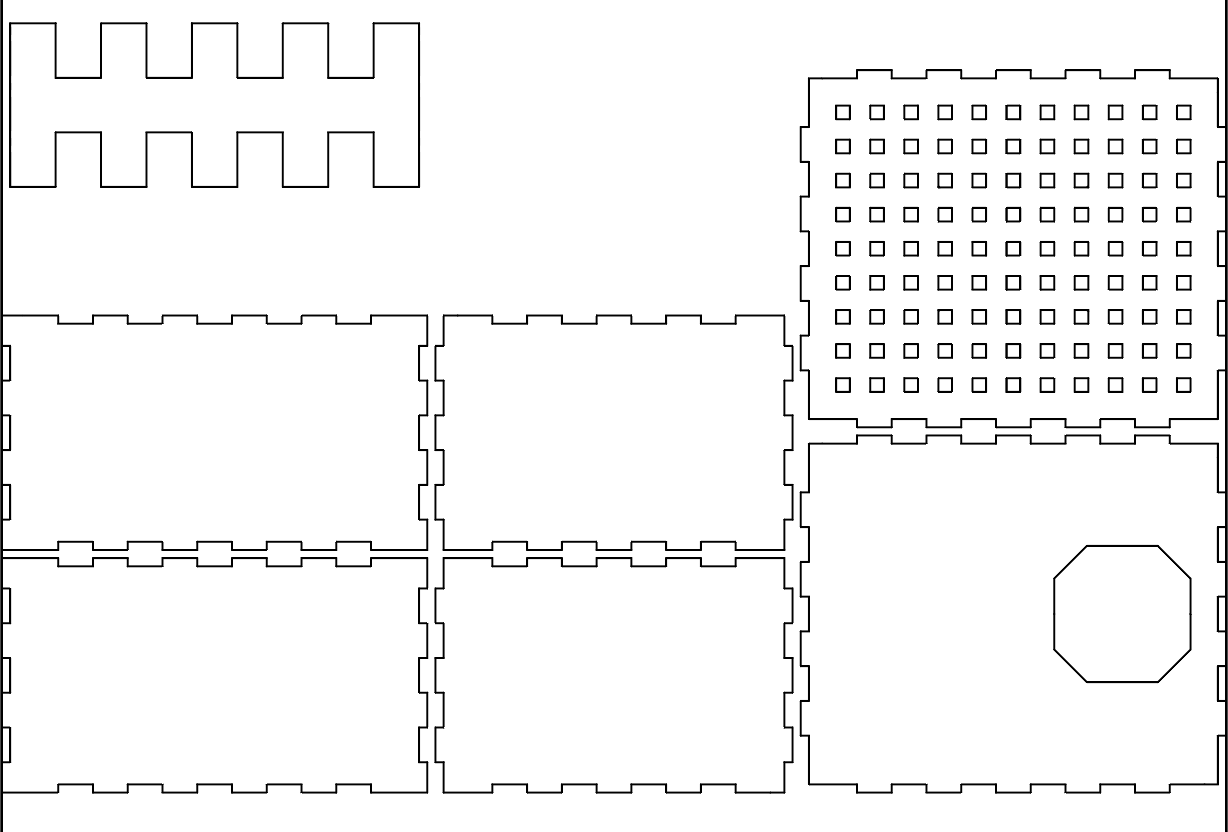
\includegraphics[width=\linewidth]{figures/dxf_mosfet_box.png}\caption{MOSFET box layout.}\end{subfigure}\hfill
\begin{subfigure}{0.32\linewidth}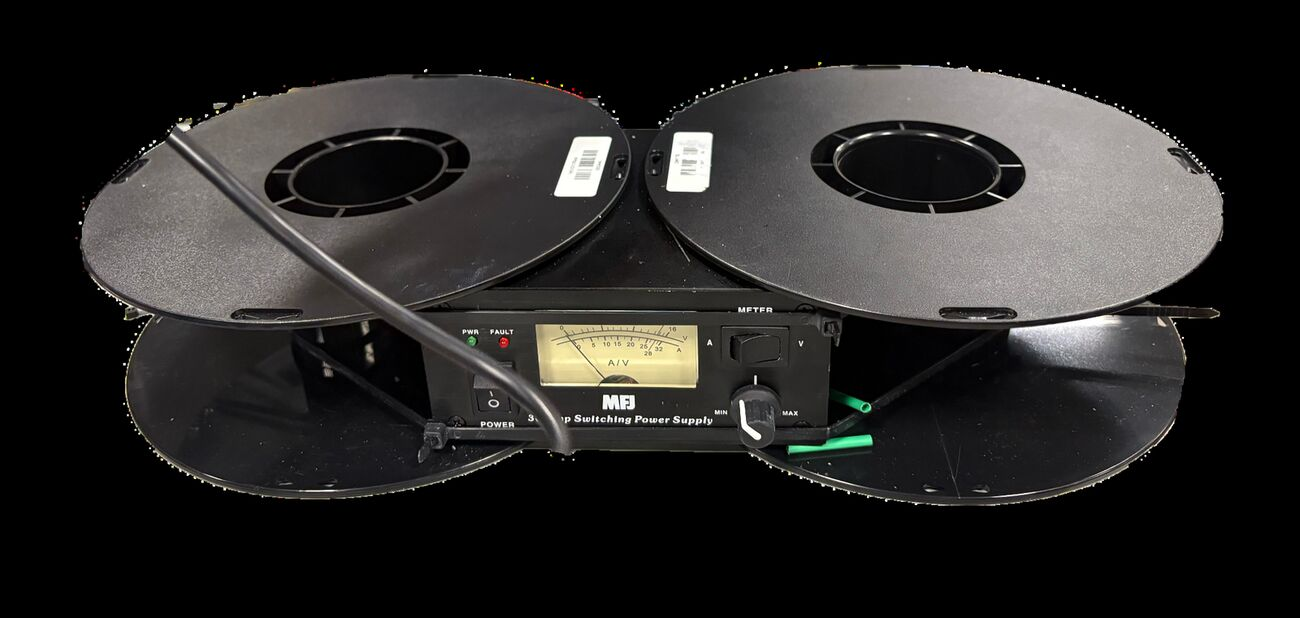
\includegraphics[width=\linewidth]{figures/psu_spools.jpg}\caption{Supply on reused spools.}\end{subfigure}
\caption{Laser-cut layouts and the supply mount.}\label{fig:encl}
\end{figure}

\section{Signal and Power Wiring}\label{sec:wiring}
\subsection{What failed first}
The first circuit drove one TEC through an IRF520 module from the Arduino, with a single fan. In extended runs the TEC hot side saturated and the MOSFET spiked in temperature. When four modules were connected, wires started to smoke (\cref{fig:wire1}).
\begin{figure}[t]\centering
\begin{subfigure}{0.40\linewidth}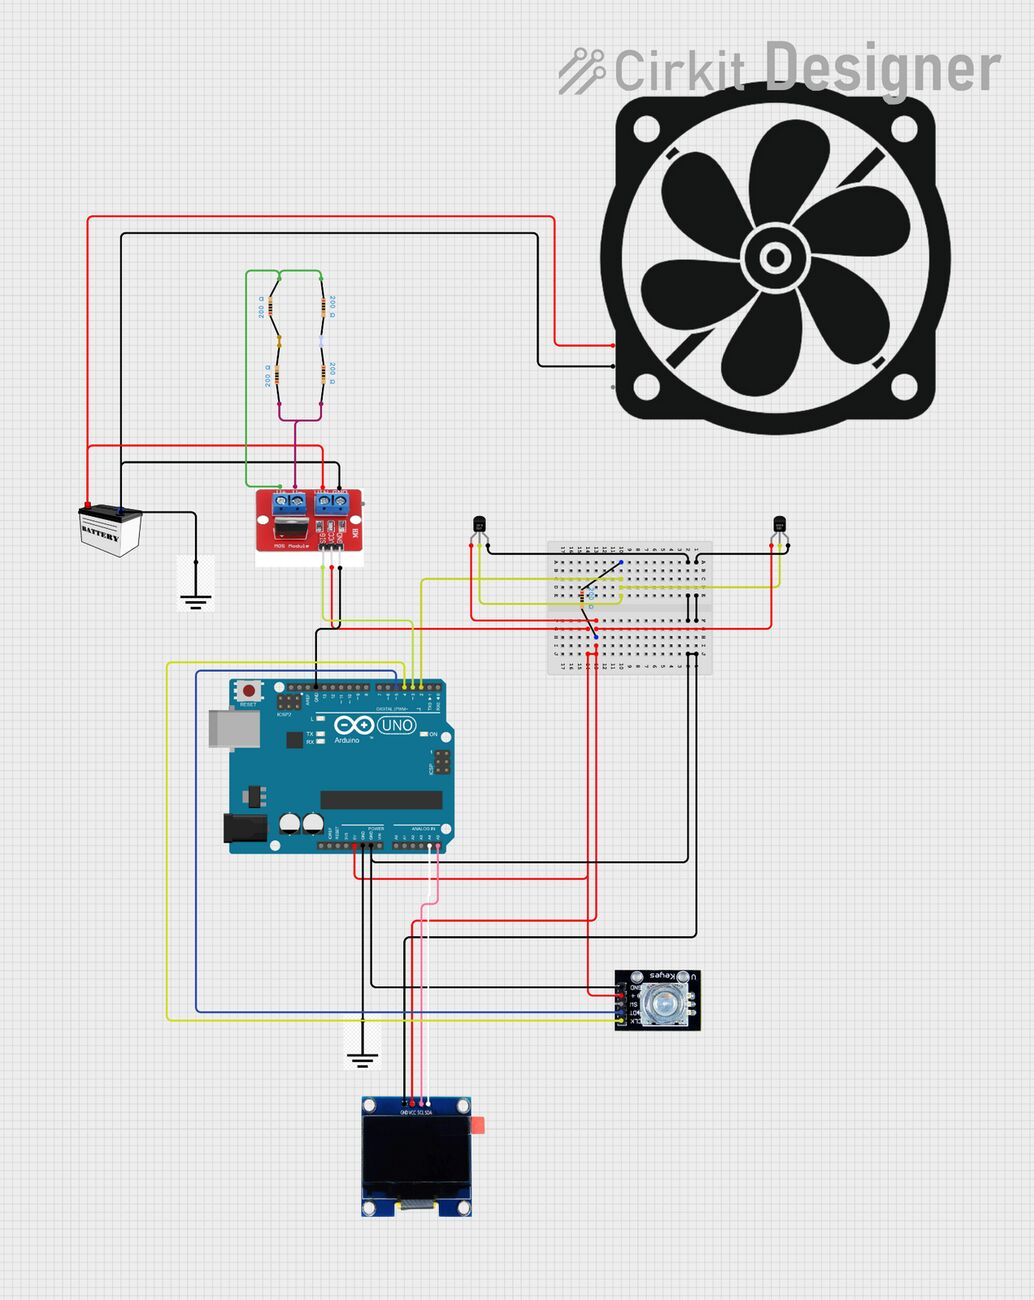
\includegraphics[width=\linewidth]{figures/circuit_v1.jpg}\caption{First circuit.}\end{subfigure}\hfill
\begin{subfigure}{0.40\linewidth}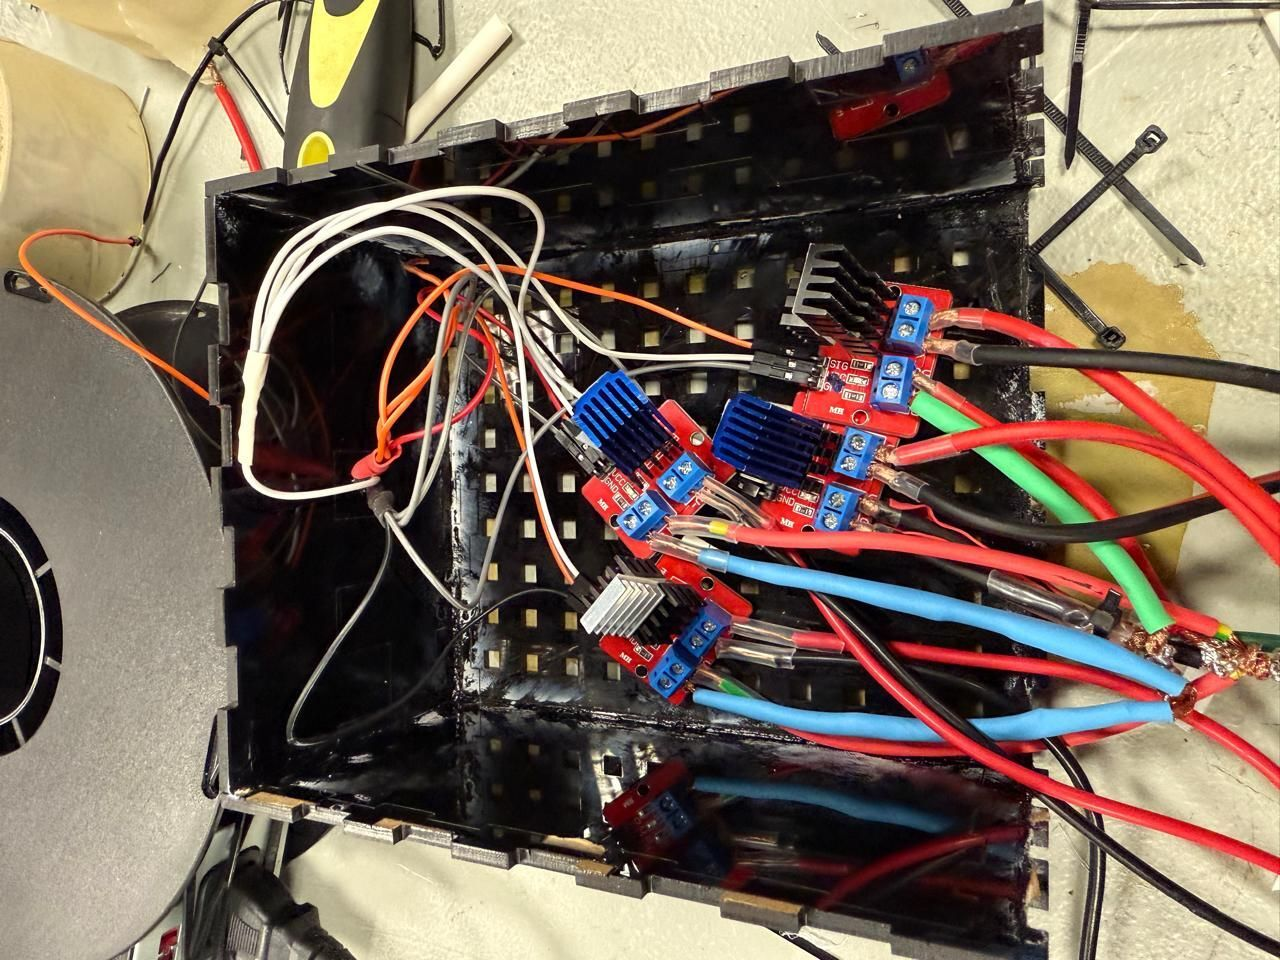
\includegraphics[width=\linewidth]{figures/wiring_smoke.jpg}\caption{Bench wiring during debugging.}\end{subfigure}
\caption{The starting point.}\label{fig:wire1}
\end{figure}

\subsection{Diagnosis}
The IRF520 reaches its quoted on-resistance of 0.27\,$\Omega$ only with about 10\,V on the gate, while an Arduino pin supplies at most about 4.5--5\,V. At that gate voltage the device sits in its linear region, so conduction loss $I^2R$ is large and the junction heats quickly at several amperes. Separately, wire gauge had not been checked against load current, and the smoking wires were a current problem. The board was crowded and had no heatsinks on the switching devices.

\subsection{Redesign}
The TEC count went from four to two in parallel, cutting total current and heat. Two IRF520 modules in parallel per TEC share the current and the conduction loss, with external heatsinks and ventilation openings. The power MOSFETs moved to their own acrylic box, physically separated from the Arduino and from the 1-wire and I$^2$C wiring, with routed and not bundled cables to limit coupling (\cref{fig:wire2}). Three fans run from the 12\,V rail for hot-side rejection; a separate power bank runs the Arduino and the two small circulation fans so cooling survives controller resets. The DS18B20 sits on the 1-wire bus on pin 2 with the standard 4.7\,k$\Omega$ pull-up.
\begin{figure}[t]\centering
\begin{subfigure}{0.60\linewidth}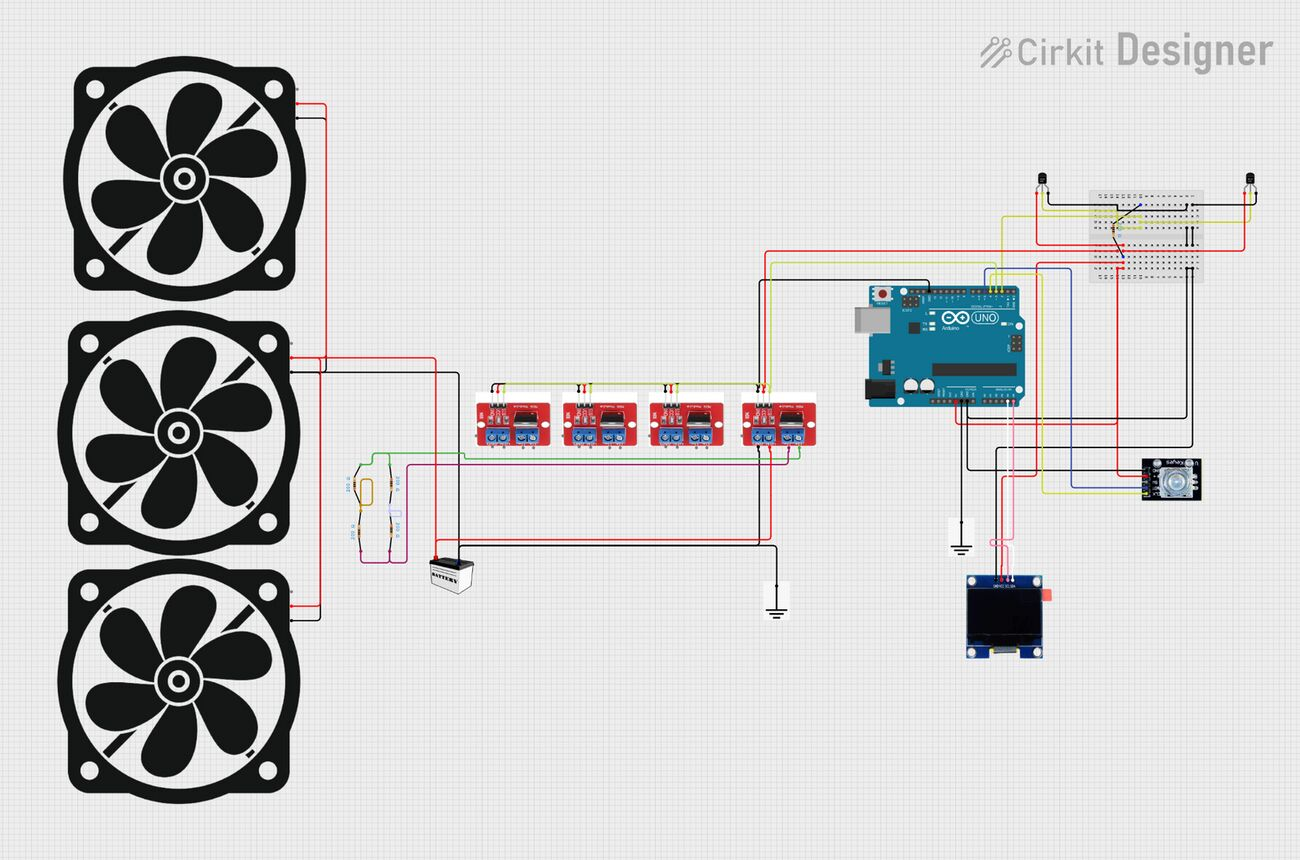
\includegraphics[width=\linewidth]{figures/circuit_v2.jpg}\caption{Modified circuit diagram.}\end{subfigure}\hfill
\begin{subfigure}{0.34\linewidth}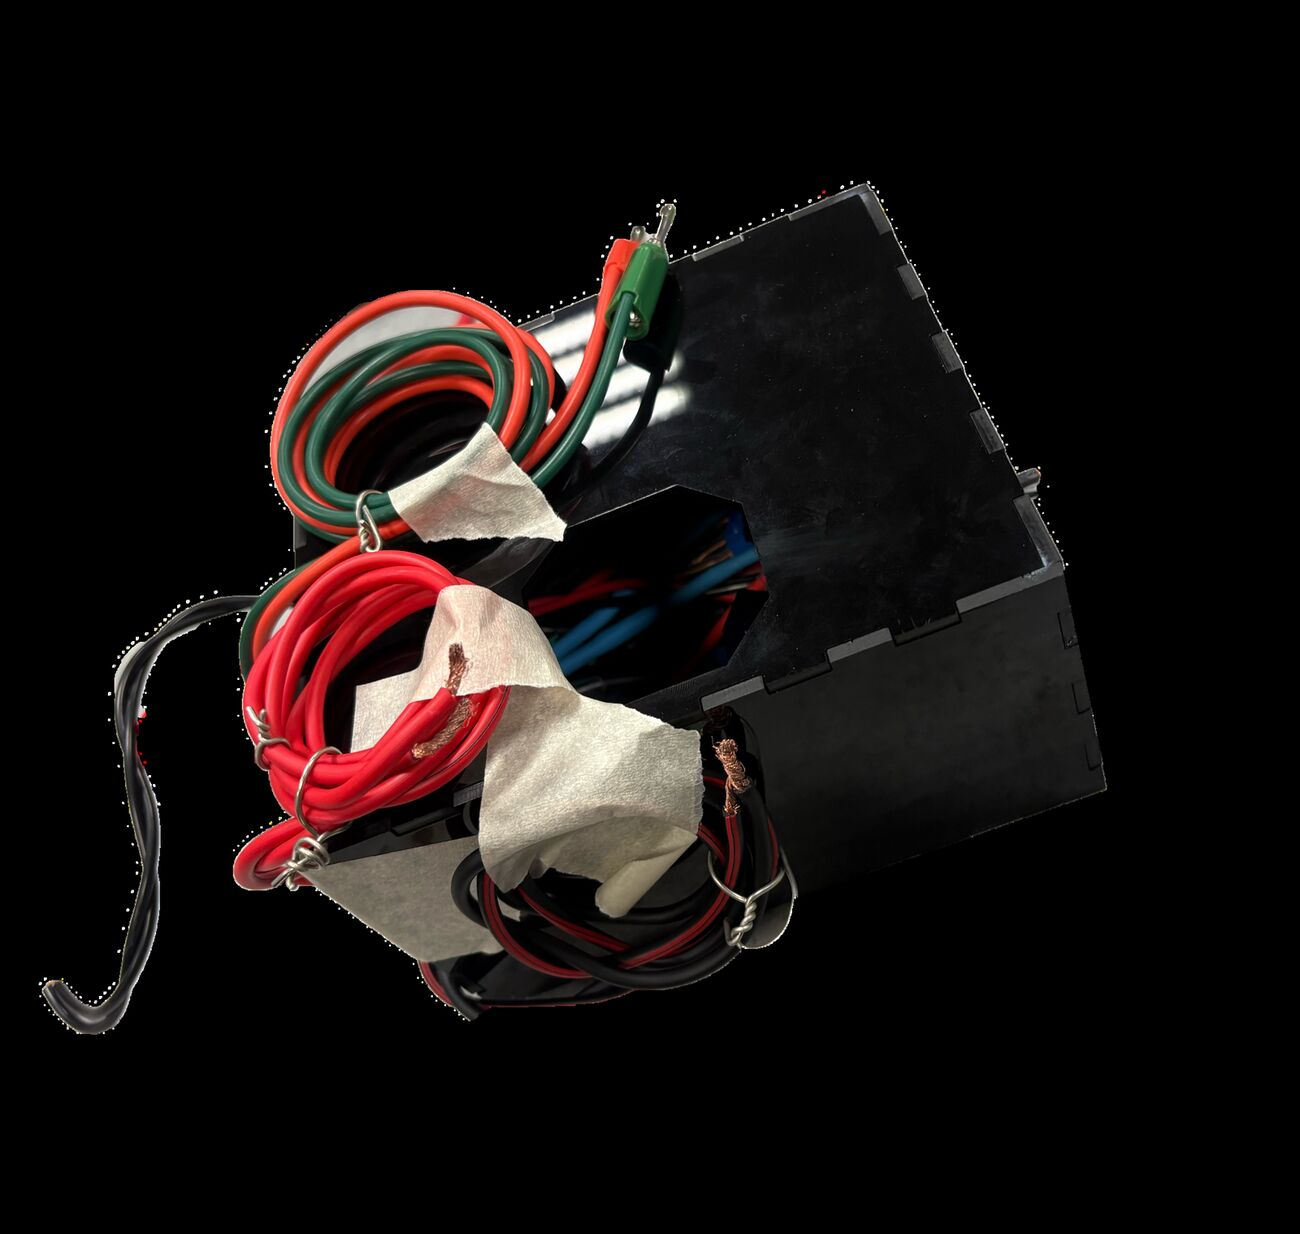
\includegraphics[width=\linewidth]{figures/mosfet_box.jpg}\caption{Isolated MOSFET box.}\end{subfigure}
\caption{Final power stage.}\label{fig:wire2}
\end{figure}
The remaining fix, which we did not build, is a logic-level MOSFET specified at $V_{GS}=4.5$\,V (an IRLZ44N or STP55NF06L) or a gate-driver IC (TC4420 or TC4427), so the device is fully enhanced from 5\,V logic. That addresses the cause and not the symptom.

\section{Results}\label{sec:results}
The cooling history of the fan-mixed chamber is in \cref{fig:cooling}. It is reconstructed from the logged time for each 1\,\textdegree C step (9, 10, 10, 11, 12--13 and about 20 minutes), not from raw data. The shrinking slope reflects falling TEC pumping capacity as the temperature difference grows.
\begin{figure}[t]\centering
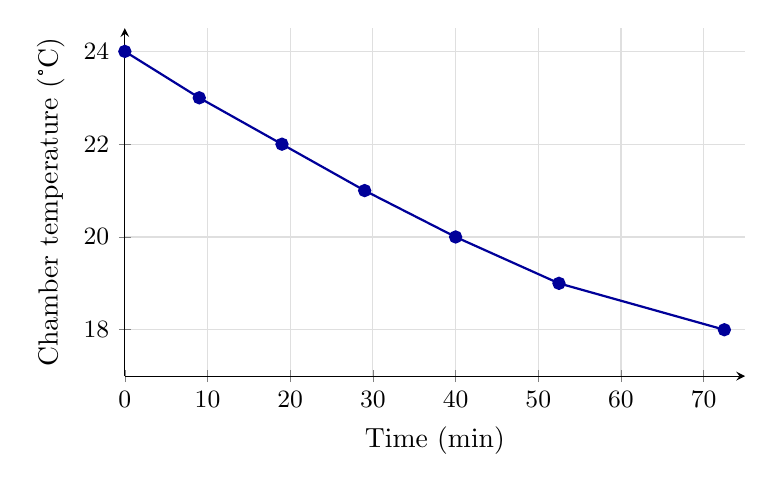
\begin{tikzpicture}
\begin{axis}[width=0.78\linewidth,height=6cm,xlabel={Time (min)},ylabel={Chamber temperature (\textdegree C)},grid=both,grid style={gray!25},ymin=17,ymax=24.5,xmin=0,xmax=75,mark size=2pt,axis lines=left,every axis plot/.append style={thick,color=blue!60!black},tick label style={font=\small}]
\addplot[mark=*] coordinates {(0,24)(9,23)(19,22)(29,21)(40,20)(52.5,19)(72.5,18)};
\end{axis}
\end{tikzpicture}
\caption{Cooling history of the fan-mixed chamber, reconstructed from logged step times.}\label{fig:cooling}
\end{figure}
\begin{table}[t]\centering\small
\begin{tabular}{@{}ll@{}}\toprule
Quantity & Result\\\midrule
Fan-mixed zone, start (ambient) to end & 24.0\,\textdegree C to 18.0\,\textdegree C\\
Zone without circulation, near the cold plate & down to 4\,\textdegree C (very local)\\
MOSFETs 1--3, steady state & 34--36\,\textdegree C\\
MOSFET 4 (highest load) & 39--40\,\textdegree C\\\bottomrule
\end{tabular}
\caption{Final prototype test results.}\label{tab:results}
\end{table}
Airflow matters. The compartment with a circulating fan reached about 12\,\textdegree C with a uniform distribution, whereas the unmixed compartment reached 4\,\textdegree C only next to the cold plate. Our test log reports both this 12\,\textdegree C reading and the stable 18.0\,\textdegree C chamber value; we use 18.0\,\textdegree C as the conservative headline. Air mixing is part of the refrigerator and not an accessory.
\begin{figure}[t]\centering
\begin{subfigure}{0.31\linewidth}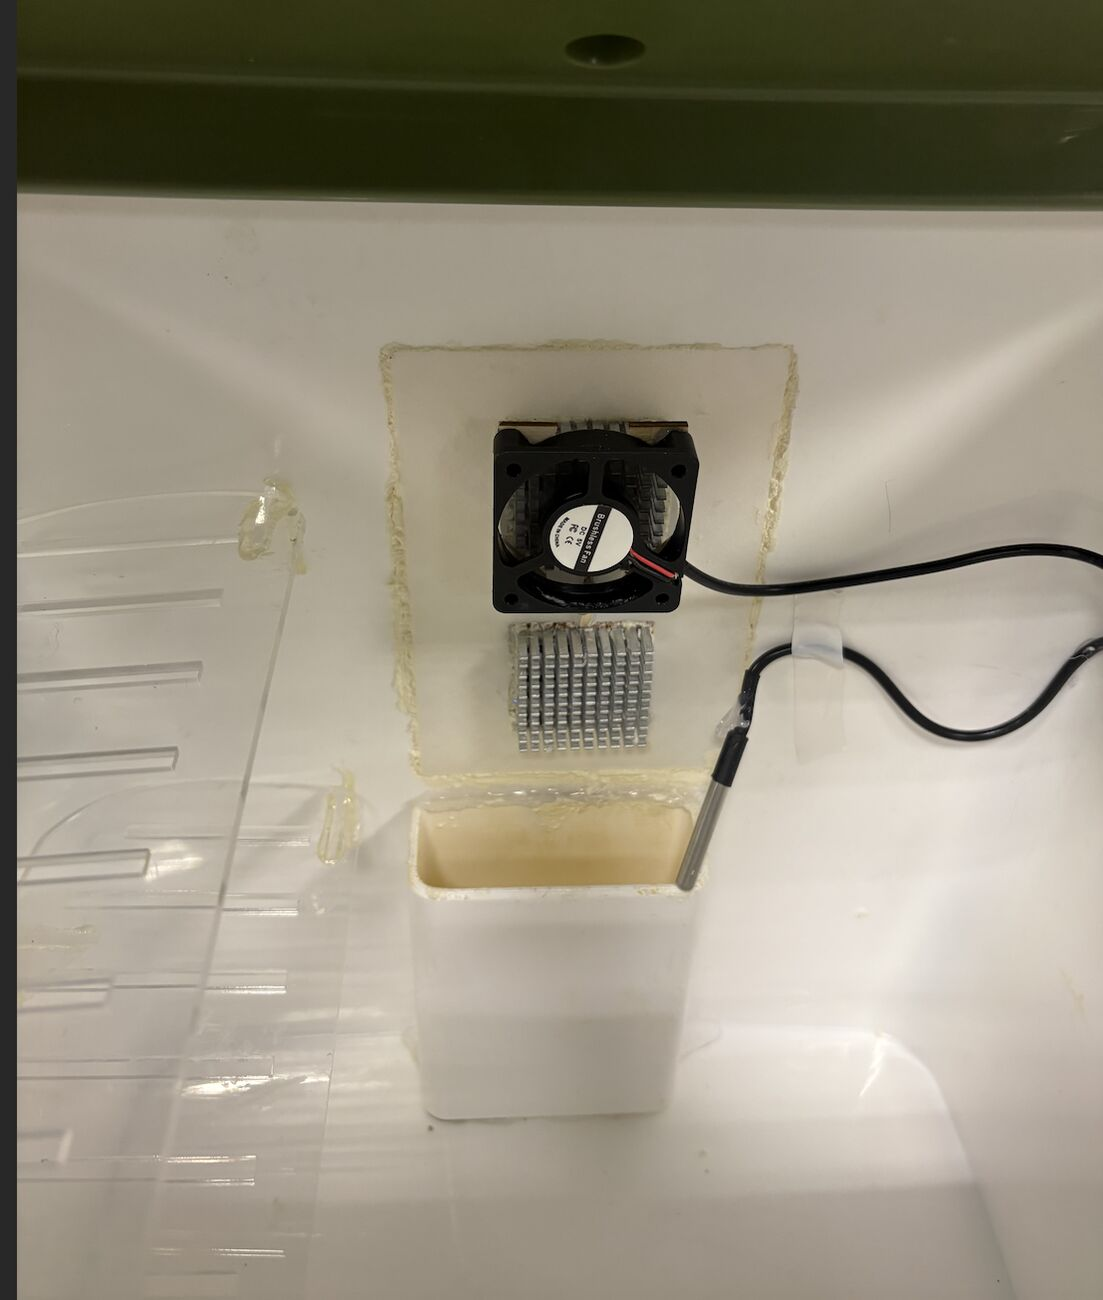
\includegraphics[width=\linewidth]{figures/inside_test.jpg}\caption{Interior test arrangement.}\end{subfigure}\hfill
\begin{subfigure}{0.31\linewidth}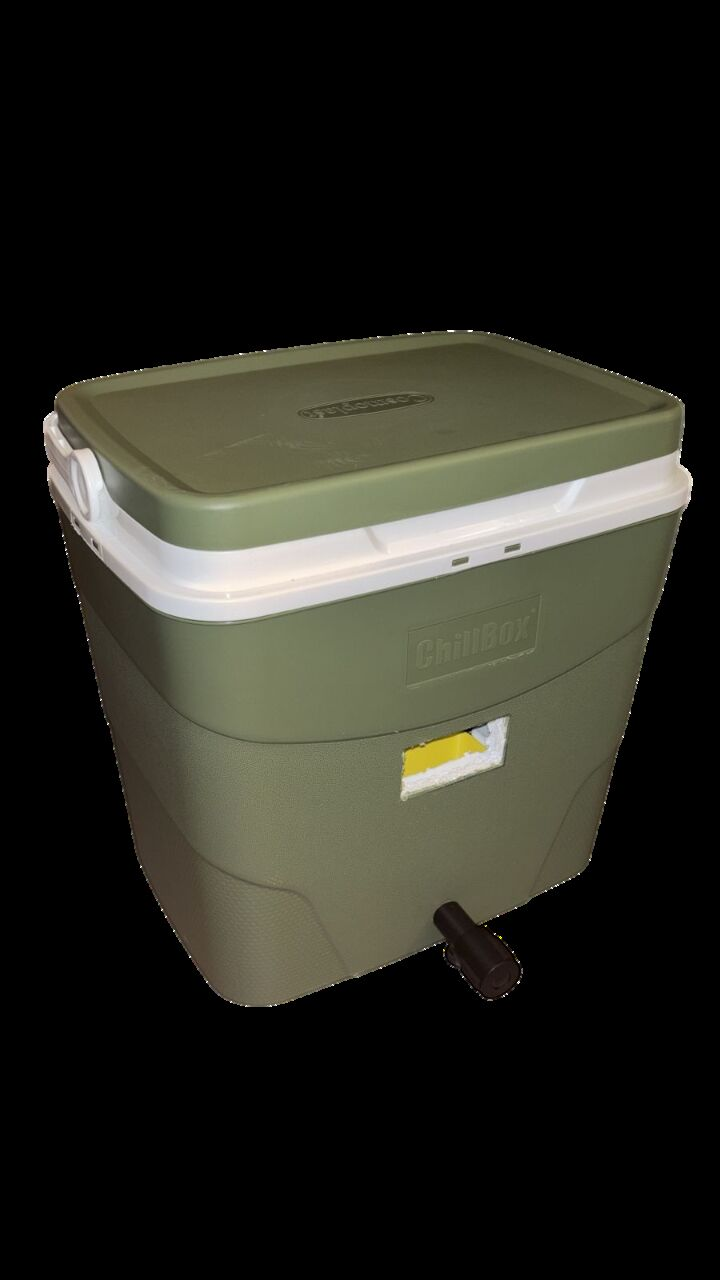
\includegraphics[width=\linewidth]{figures/cooler.jpg}\caption{Cooler with valve.}\end{subfigure}\hfill
\begin{subfigure}{0.31\linewidth}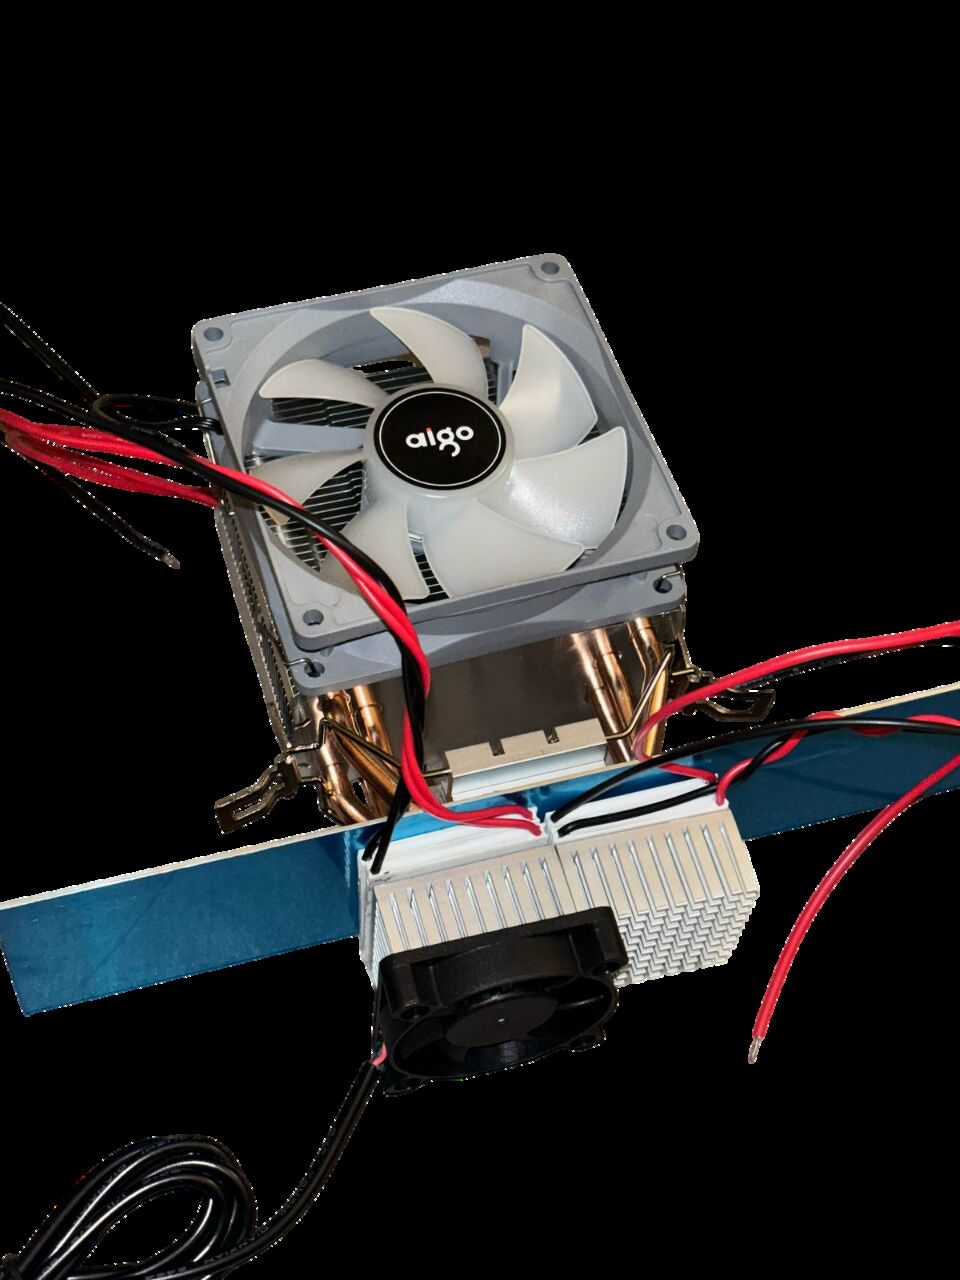
\includegraphics[width=\linewidth]{figures/tec_photo.jpg}\caption{Early TEC and fan stack.}\end{subfigure}
\caption{Prototype photographs.}\label{fig:photos}
\end{figure}

\section{Discussion}\label{sec:discussion}
\textbf{Why the target was missed.} The sub-10\,\textdegree C goal was not reached. In order of impact: the heat-rejection capacity of the TEC stack, a MOSFET drive that limited the usable current, and initially poor internal air mixing. The first is physics, since the cold-side capacity depends on how cool the hot side is kept; the second is a component choice.

\textbf{Practical consequences.} If we built it again we would use larger finned or liquid-cooled hot-side exchangers, fix the gate drive, move to the conventional PID form with a filtered, non-blocking sensor read and automated tuning, and hold the TEC stack with spring-loaded clamps for uniform pressure.

\textbf{What this study does not establish.} The cooling curve is reconstructed from step times. No controlled comparison of print materials was run: choices came from datasheet limits and build experience, and a study of PLA against PETG or of infill with thermal measurements would be the right next step. The reference sketch in the repository uses the conventional \texttt{REVERSE} form and was reconstructed from the documented configuration; it was not run on the original hardware, and the OLED and encoder are replaced by a serial setpoint command. Whether the conventional form changes the erratic regime has not been tested. The recommended gate-drive fix has not been built.

\textbf{Conclusion.} A Peltier cooler built from commodity parts reached 18.0\,\textdegree C from 24.0\,\textdegree C once the hot side was given its own fans and platform and the MOSFETs were isolated and doubled. The PID gains were found by observing how each ordering failed. Missing the 10\,\textdegree C goal was a heat-rejection and gate-drive problem, and both have identified fixes.

\section*{Code and data availability}
The control sketch, the report source and the figures are in the repository accompanying it. The reference sketch is in \texttt{firmware/tec\_pid}.

\bibliographystyle{plainnat}
\bibliography{references}
\end{document}
